% ============================================================
%  SCHOLA DOMESTICA — Magister Mathematica
%  Level 1 | Week 5 | Day 3
%  Topic: Ordering Numbers 0–10 — Before, After, Between
%  Enrichment: Roman Numerals VI–X (fill-in sequence)
% ============================================================
\documentclass[12pt, letterpaper]{article}

\usepackage[top=1in, bottom=1in, left=1in, right=1in]{geometry}
\usepackage{fontenc}
\usepackage{inputenc}
\usepackage{lmodern}
\usepackage{microtype}
\usepackage{amsmath}
\usepackage{graphicx}
\usepackage{xcolor}
\usepackage{tikz}
\usepackage{array}
\usepackage{enumitem}
\usepackage{multicol}
\usepackage{mdframed}
\usepackage{fancyhdr}

\definecolor{scholared}{RGB}{160,30,30}
\definecolor{scholagold}{RGB}{180,140,40}
\definecolor{scholacream}{RGB}{253,248,235}
\definecolor{scholagreen}{RGB}{50,110,60}
\definecolor{scholablue}{RGB}{40,80,140}

\pagestyle{fancy}
\fancyhf{}
\renewcommand{\headrulewidth}{0.6pt}
\fancyhead[L]{\small\textcolor{scholared}{\textbf{Schola Domestica — Magister Mathematica}}}
\fancyhead[R]{\small\textcolor{scholared}{Level 1 · Week 5 · Day 3}}
\fancyfoot[C]{\small\textcolor{gray}{— \thepage\ —}}

\newcommand{\answerline}{\underline{\hspace{2.5cm}}}
\newcommand{\biganswerline}{\underline{\hspace{4cm}}}
\newcommand{\numbox}{\fbox{\hspace{0.6cm}\vphantom{0}}}

\newmdenv[
  backgroundcolor=scholacream,
  linecolor=scholared,
  linewidth=1.5pt,
  roundcorner=6pt,
  innertopmargin=8pt,
  innerbottommargin=8pt,
  innerleftmargin=10pt,
  innerrightmargin=10pt
]{lessonbox}

\begin{document}

\begin{center}
  {\LARGE\textbf{\textcolor{scholared}{Ordering Numbers 0–10}}}\\[4pt]
  {\Large\textcolor{scholagold}{\textit{Before, After, and Between}}}\\[6pt]
  {\small Name: \biganswerline \hspace{1cm} Date: \answerline}
\end{center}

\vspace{4pt}
\noindent\textcolor{scholared}{\rule{\linewidth}{1pt}}
\vspace{4pt}

% IMAGE PROMPT (Beatrix Potter watercolour style):
% A wooden garden fence with 11 numbered posts (0 through 10), each post a slightly different
% height. A row of goldfinches is perched on the fence, each bird sitting on one post.
% Soft watercolour, sunny morning light, green meadow behind. No text in image.

\begin{lessonbox}
\textbf{The Number Line:}\\[4pt]
Numbers live in order on a line. Each number has a \textbf{before} and an \textbf{after}.\\[6pt]
\begin{center}
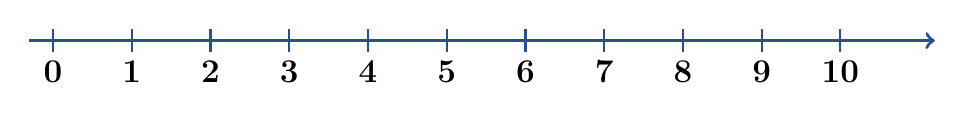
\begin{tikzpicture}[scale=1]
  % number line
  \draw[very thick, scholablue, ->] (-0.3,0) -- (11.2,0);
  \foreach \n in {0,...,10} {
    \draw[thick, scholablue] (\n,0.15) -- (\n,-0.15);
    \node[below=4pt] at (\n,0) {\large\textbf{\n}};
  }
\end{tikzpicture}
\end{center}
\medskip
\noindent\textit{The number just before 7 is} \textbf{6}. \quad
\textit{The number just after 7 is} \textbf{8}. \quad
\textit{7 is between 6 and 8.}
\end{lessonbox}

\bigskip

% ===== PART I: BEFORE AND AFTER =====
\noindent\textcolor{scholared}{\large\textbf{Part I — Before and After}} \hfill \textit{(Problems 1–6)}

\medskip
\noindent\textit{Write the number that comes \textbf{just before} and \textbf{just after}.}

\bigskip

\begin{multicols}{2}
\noindent\textbf{1.} \quad \numbox \; , \; \textbf{6} \; , \; \numbox \\[16pt]
\noindent\textbf{2.} \quad \numbox \; , \; \textbf{9} \; , \; \numbox \\[16pt]
\noindent\textbf{3.} \quad \numbox \; , \; \textbf{7} \; , \; \numbox

\columnbreak

\noindent\textbf{4.} \quad \numbox \; , \; \textbf{10} \; , \; \numbox \\[16pt]
\noindent\textbf{5.} \quad \numbox \; , \; \textbf{8} \; , \; \numbox \\[16pt]
\noindent\textbf{6.} \quad \numbox \; , \; \textbf{0} \; , \; \numbox
\end{multicols}

\medskip
\noindent{\small\textit{(Hint for problem 6: there is no number before 0.)}}

\bigskip
\noindent\textcolor{scholared}{\rule{\linewidth}{0.4pt}}

% ===== PART II: BETWEEN =====
\noindent\textcolor{scholared}{\large\textbf{Part II — What is Between?}} \hfill \textit{(Problems 7–10)}

\medskip
\noindent\textit{Write the missing number that belongs \textbf{between} the two numbers shown.}

\bigskip
\noindent\textbf{7.} \quad 6 \; , \; \numbox \; , \; 8 \\[16pt]
\noindent\textbf{8.} \quad 8 \; , \; \numbox \; , \; 10 \\[16pt]
\noindent\textbf{9.} \quad 5 \; , \; \numbox \; , \; 7 \\[16pt]
\noindent\textbf{10.} \quad 0 \; , \; \numbox \; , \; 2

\bigskip
\noindent\textcolor{scholared}{\rule{\linewidth}{0.4pt}}

% ===== PART III: FILL THE NUMBER LINE =====
\noindent\textcolor{scholared}{\large\textbf{Part III — Fill the Number Line}} \hfill \textit{(Problem 11)}

\bigskip
\noindent\textit{Some numbers are missing. Write them in the boxes.}

\bigskip
\begin{center}
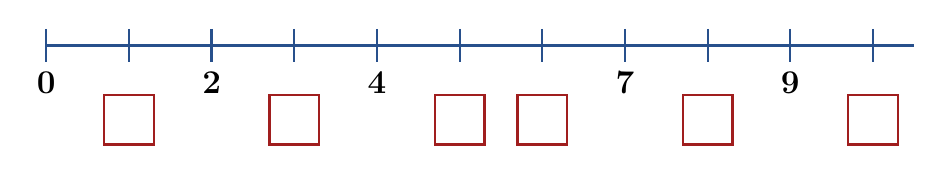
\begin{tikzpicture}[scale=1.05]
  \draw[very thick, scholablue] (0,0) -- (10.5,0);
  % ticks
  \foreach \n in {0,...,10} {
    \draw[thick, scholablue] (\n, 0.2) -- (\n,-0.2);
  }
  % provided numbers
  \node[below=6pt] at (0,0) {\large\textbf{0}};
  \node[below=6pt] at (2,0) {\large\textbf{2}};
  \node[below=6pt] at (4,0) {\large\textbf{4}};
  \node[below=6pt] at (7,0) {\large\textbf{7}};
  \node[below=6pt] at (9,0) {\large\textbf{9}};
  % blank boxes
  \foreach \n in {1,3,5,6,8,10} {
    \draw[thick, scholared] (\n-0.3,-0.6) rectangle (\n+0.3,-1.2);
  }
\end{tikzpicture}
\end{center}

\bigskip
\noindent\textcolor{scholared}{\rule{\linewidth}{0.4pt}}

% ===== PART IV: KNOWLEDGE CHECK =====
\noindent\textcolor{scholared}{\large\textbf{Part IV — Knowledge Check}} \hfill \textit{(Problems 12–14)}

\bigskip
\noindent\textbf{12.} What number comes just before 10? \hfill \answerline

\bigskip
\noindent\textbf{13.} What number is between 6 and 8? \hfill \answerline

\bigskip
\noindent\textbf{14.} Write all the numbers from 6 to 10 in order:

\medskip
\hspace{2em}\numbox \; , \; \numbox \; , \; \numbox \; , \; \numbox \; , \; \numbox

\bigskip
\noindent\textcolor{scholared}{\rule{\linewidth}{0.4pt}}

% ===== ENRICHMENT =====
\begin{lessonbox}
\textcolor{scholared}{\textbf{Enrichment — Roman Numeral Sequence}}\\[6pt]
\noindent Fill in the missing Roman numerals. The first one is done for you.\\[8pt]
\begin{center}
\renewcommand{\arraystretch}{1.6}
\begin{tabular}{|c|c|c|c|c|c|c|c|c|c|}
\hline
\textbf{I} & \textbf{II} & \textbf{III} & \textbf{IV} & \textbf{V} & \fbox{\hspace{0.5cm}} & \fbox{\hspace{0.5cm}} & \fbox{\hspace{0.5cm}} & \fbox{\hspace{0.5cm}} & \fbox{\hspace{0.5cm}} \\
\hline
1 & 2 & 3 & 4 & 5 & 6 & 7 & 8 & 9 & 10 \\
\hline
\end{tabular}
\end{center}
\end{lessonbox}

\end{document}
